
%%% Preamble
\documentclass[paper=a4, fontsize=11pt]{scrartcl}


\usepackage{float}
%\usepackage{geometry} %AGREGOOOOO
%\geometry{verbose,tmargin=2cm,bmargin=2cm,lmargin=2cm,rmargin=2cm,headheight=2cm,headsep=2cm}
%\geometry{verbose,tmargin=2cm,bmargin=2cm,lmargin=2cm,rmargin=2cm,headheight=2cm,headsep=2cm}
\usepackage{multirow}



\usepackage[T1]{fontenc}
\usepackage{fourier}
\usepackage[utf8]{inputenc}
\usepackage[english]{babel}					% English language/hyphenation

\usepackage[protrusion=true,expansion=true]{microtype}	
\usepackage{amsmath,amsfonts,amsthm} % Math packages
\usepackage[pdftex]{graphicx}	
\usepackage{url} %SACO ESTO
\usepackage{import}

\usepackage[margin=2cm]{geometry}
\geometry{verbose,tmargin=2cm,bmargin=2cm,lmargin=2cm,rmargin=2cm,headheight=2cm,headsep=2cm} %SACO ESTO
% %%% Custom sectioning
\usepackage{sectsty}
\allsectionsfont{\normalfont \scshape}


%%COMENTO ESTO

%%% Custom headers/footers (fancyhdr package)
%\usepackage{fancyhdr}
%\pagestyle{fancyplain}
%\fancyhead{}											% No page header
%\fancyfoot[L]{}											% Empty 
%\fancyfoot[C]{}											% Empty
%\fancyfoot[R]{\thepage}									% Pagenumbering
%\renewcommand{\headrulewidth}{0pt}			% Remove header underlines
%\renewcommand{\footrulewidth}{0pt}				% Remove footer underlines
%\setlength{\headheight}{13.6pt}




%%% Equation and float numbering
\numberwithin{equation}{section}		% Equationnumbering: section.eq#
\numberwithin{figure}{section}			% Figurenumbering: section.fig#
\numberwithin{table}{section}				% Tablenumbering: section.tab#


%%% Maketitle metadata
\newcommand{\horrule}[1]{\rule{\linewidth}{#1}} 	% Horizontal rule

%AGREGO PARA EJ 1
\usepackage{graphicx}
\usepackage{color} 
\usepackage[dvipsnames]{xcolor}
\colorlet{purple}{purple}

%/////////////////////////////////// AGREGO PARA EL EJ 2

    \usepackage{geometry} % Required to change the page size to A4
    \geometry{a4paper} % Set the page size to be A4 as opposed to the default US Letter

    \usepackage{mathtools, nccmath}
     
    
    
%%%%%%%%%%%%% AGREGOOOOO
\usepackage{xcolor}



    \usepackage{tikz}
    \usetikzlibrary{matrix,calc}

    %isolated term
%#1 - Optional. Space between node and grouping line. Default=0
%#2 - node
%#3 - filling color
\newcommand{\implicantsol}[3][0]{
    \draw[rounded corners=3pt, fill=#3, opacity=0.3] ($(#2.north west)+(135:#1)$) rectangle ($(#2.south east)+(-45:#1)$);
    }


%internal group
%#1 - Optional. Space between node and grouping line. Default=0
%#2 - top left node
%#3 - bottom right node
%#4 - filling color
\newcommand{\implicant}[4][0]{
    \draw[rounded corners=3pt, fill=#4, opacity=0.3] ($(#2.north west)+(135:#1)$) rectangle ($(#3.south east)+(-45:#1)$);
    }

%group lateral borders
%#1 - Optional. Space between node and grouping line. Default=0
%#2 - top left node
%#3 - bottom right node
%#4 - filling color
\newcommand{\implicantcostats}[4][0]{
    \draw[rounded corners=3pt, fill=#4, opacity=0.3] ($(rf.east |- #2.north)+(90:#1)$)-| ($(#2.east)+(0:#1)$) |- ($(rf.east |- #3.south)+(-90:#1)$);
    \draw[rounded corners=3pt, fill=#4, opacity=0.3] ($(cf.west |- #2.north)+(90:#1)$) -| ($(#3.west)+(180:#1)$) |- ($(cf.west |- #3.south)+(-90:#1)$);
}

%group top-bottom borders
%#1 - Optional. Space between node and grouping line. Default=0
%#2 - top left node
%#3 - bottom right node
%#4 - filling color
\newcommand{\implicantdaltbaix}[4][0]{
    \draw[rounded corners=3pt, fill=#4, opacity=0.3] ($(cf.south -| #2.west)+(180:#1)$) |- ($(#2.south)+(-90:#1)$) -| ($(cf.south -| #3.east)+(0:#1)$);
    \draw[rounded corners=3pt, fill=#4, opacity=0.3] ($(rf.north -| #2.west)+(180:#1)$) |- ($(#3.north)+(90:#1)$) -| ($(rf.north -| #3.east)+(0:#1)$);
}

%group corners
%#1 - Optional. Space between node and grouping line. Default=0
%#2 - filling color
\newcommand{\implicantcantons}[2][0]{
    \draw[rounded corners=3pt, opacity=.3] ($(rf.east |- 0.south)+(-90:#1)$) -| ($(0.east |- cf.south)+(0:#1)$);
    \draw[rounded corners=3pt, opacity=.3] ($(rf.east |- 8.north)+(90:#1)$) -| ($(8.east |- rf.north)+(0:#1)$);
    \draw[rounded corners=3pt, opacity=.3] ($(cf.west |- 2.south)+(-90:#1)$) -| ($(2.west |- cf.south)+(180:#1)$);
    \draw[rounded corners=3pt, opacity=.3] ($(cf.west |- 10.north)+(90:#1)$) -| ($(10.west |- rf.north)+(180:#1)$);
    \fill[rounded corners=3pt, fill=#2, opacity=.3] ($(rf.east |- 0.south)+(-90:#1)$) -|  ($(0.east |- cf.south)+(0:#1)$) [sharp corners] ($(rf.east |- 0.south)+(-90:#1)$) |-  ($(0.east |- cf.south)+(0:#1)$) ;
    \fill[rounded corners=3pt, fill=#2, opacity=.3] ($(rf.east |- 8.north)+(90:#1)$) -| ($(8.east |- rf.north)+(0:#1)$) [sharp corners] ($(rf.east |- 8.north)+(90:#1)$) |- ($(8.east |- rf.north)+(0:#1)$) ;
    \fill[rounded corners=3pt, fill=#2, opacity=.3] ($(cf.west |- 2.south)+(-90:#1)$) -| ($(2.west |- cf.south)+(180:#1)$) [sharp corners]($(cf.west |- 2.south)+(-90:#1)$) |- ($(2.west |- cf.south)+(180:#1)$) ;
    \fill[rounded corners=3pt, fill=#2, opacity=.3] ($(cf.west |- 10.north)+(90:#1)$) -| ($(10.west |- rf.north)+(180:#1)$) [sharp corners] ($(cf.west |- 10.north)+(90:#1)$) |- ($(10.west |- rf.north)+(180:#1)$) ;
}

%Empty Karnaugh map 4x4
\newenvironment{Karnaugh}%
{
\begin{tikzpicture}[baseline=(current bounding box.north),scale=0.8]
\draw (0,0) grid (4,4);
\draw (0,4) -- node [pos=0.7,above right,anchor=south west] {y2 y1} node [pos=0.75,below left,anchor=north east] {w y3} ++(135:1);
%
\matrix (mapa) [matrix of nodes,
        column sep={0.8cm,between origins},
        row sep={0.8cm,between origins},
        every node/.style={minimum size=0.3mm},
        anchor=8.center,
        ampersand replacement=\&] at (0.5,0.5)
{
                       \& |(c00)| 00         \& |(c01)| 01         \& |(c11)| 11         \& |(c10)| 10         \& |(cf)| \phantom{00} \\
|(r00)| 00             \& |(0)|  \phantom{0} \& |(1)|  \phantom{0} \& |(3)|  \phantom{0} \& |(2)|  \phantom{0} \&                     \\
|(r01)| 01             \& |(4)|  \phantom{0} \& |(5)|  \phantom{0} \& |(7)|  \phantom{0} \& |(6)|  \phantom{0} \&                     \\
|(r11)| 11             \& |(12)| \phantom{0} \& |(13)| \phantom{0} \& |(15)| \phantom{0} \& |(14)| \phantom{0} \&                     \\
|(r10)| 10             \& |(8)|  \phantom{0} \& |(9)|  \phantom{0} \& |(11)| \phantom{0} \& |(10)| \phantom{0} \&                     \\
|(rf) | \phantom{00}   \&                    \&                    \&                    \&                    \&                     \\
};
}%
{
\end{tikzpicture}
}

%Empty Karnaugh map 2x4
\newenvironment{Karnaughvuit}%
{
\begin{tikzpicture}[baseline=(current bounding box.north),scale=0.8]
\draw (0,0) grid (4,2);
\draw (0,2) -- node [pos=0.7,above right,anchor=south west] {y2 y1} node [pos=0.7,below left,anchor=north east] {y3} ++(135:1);
%
\matrix (mapa) [matrix of nodes,
        column sep={0.8cm,between origins},
        row sep={0.8cm,between origins},
        every node/.style={minimum size=0.3mm},
        anchor=4.center,
        ampersand replacement=\&] at (0.5,0.5)
{
                      \& |(c00)| 00         \& |(c01)| 01         \& |(c11)| 11         \& |(c10)| 10         \& |(cf)| \phantom{00} \\
|(r00)| 0             \& |(0)|  \phantom{0} \& |(1)|  \phantom{0} \& |(3)|  \phantom{0} \& |(2)|  \phantom{0} \&                     \\
|(r01)| 1             \& |(4)|  \phantom{0} \& |(5)|  \phantom{0} \& |(7)|  \phantom{0} \& |(6)|  \phantom{0} \&                     \\
|(rf) | \phantom{00}  \&                    \&                    \&                    \&                    \&                     \\
};
}%
{
\end{tikzpicture}
}

%Empty Karnaugh map 2x2
\newenvironment{Karnaughquatre}%
{
\begin{tikzpicture}[baseline=(current bounding box.north),scale=0.8]
\draw (0,0) grid (2,2);
\draw (0,2) -- node [pos=0.7,above right,anchor=south west] {b} node [pos=0.7,below left,anchor=north east] {a} ++(135:1);
%
\matrix (mapa) [matrix of nodes,
        column sep={0.8cm,between origins},
        row sep={0.8cm,between origins},
        every node/.style={minimum size=0.3mm},
        anchor=2.center,
        ampersand replacement=\&] at (0.5,0.5)
{
          \& |(c00)| 0          \& |(c01)| 1  \\
|(r00)| 0 \& |(0)|  \phantom{0} \& |(1)|  \phantom{0} \\
|(r01)| 1 \& |(2)|  \phantom{0} \& |(3)|  \phantom{0} \\
};
}%
{
\end{tikzpicture}
}

%Defines 8 or 16 values (0,1,X)
\newcommand{\contingut}[1]{%
\foreach \x [count=\xi from 0]  in {#1}
     \path (\xi) node {\x};
}

%Places 1 in listed positions
\newcommand{\minterms}[1]{%
    \foreach \x in {#1}
        \path (\x) node {1};
}

%Places 0 in listed positions
\newcommand{\maxterms}[1]{%
    \foreach \x in {#1}
        \path (\x) node {0};
}

%Places X in listed positions
\newcommand{\indeterminats}[1]{%
    \foreach \x in {#1}
        \path (\x) node {X};
}

    \linespread{1.2} % Line spacing
    
    \setlength\parindent{0pt} % Uncomment to remove all indentation from paragraphs
    
   % \graphicspath{{/home/bzerol/VisualCode/ElectroIII/tp1-team-2/E2TP1}} % Specifies the directory where pictures are stored

%//////////////////////////////////// agrego para EJ 4
%\documentclass[english]{article}
%\usepackage[T1]{fontenc}
%\usepackage[latin9]{inputenc}
%\usepackage{geometry}
%\geometry{verbose,tmargin=2cm,bmargin=2cm,lmargin=2cm,rmargin=2cm,headheight=2cm,headsep=2cm}
%\usepackage{float}
%\usepackage{graphicx}

\makeatletter

%%%%%%%%%%%%%%%%%%%%%%%%%%%%%% LyX specific LaTeX commands.
%% Because html converters don't know tabularnewline
\providecommand{\tabularnewline}{\\}

%%%%%%%%%%%%%%%%%%%%%%%%%%%%%% User specified LaTeX commands.
\usepackage{babel}


\makeatother

\usepackage{babel}

%///////////////////////////// PARA EL EJ6
%\documentclass[english]{article}
%\usepackage[T1]{fontenc}
%\usepackage[latin9]{inputenc}
%\usepackage{geometry}
%\geometry{verbose,tmargin=3cm,bmargin=3cm,lmargin=3cm,rmargin=3cm,headheight=3cm,headsep=3cm}
%\usepackage{float}

%\makeatletter

%%%%%%%%%%%%%%%%%%%%%%%%%%%%%% LyX specific LaTeX commands.
%% Because html converters don't know tabularnewline
\providecommand{\tabularnewline}{\\}



%%AGREG0 
\usepackage{tikz}
\usetikzlibrary{shapes,arrows}

\tikzstyle{decision} = [diamond, draw, fill=blue!20, 
    text width=4.5em, text badly centered, node distance=4cm, inner sep=0pt]
\tikzstyle{block} = [rectangle, draw, fill=blue!20, 
    text width=5em, text centered, rounded corners, minimum height=2em]
\tikzstyle{line} = [draw, -latex']
\tikzstyle{cloud} = [draw, ellipse,fill=red!20, node distance=3cm,
    minimum height=2em]

\usepackage{listings}

\usepackage[utf8]{inputenc}
 
\usepackage{listings}
%\usepackage{color}
 
\definecolor{codegreen}{rgb}{0,0.6,0}
\definecolor{codegray}{rgb}{0.5,0.5,0.5}
\definecolor{codepurple}{rgb}{0.58,0,0.82}
\definecolor{backcolour}{rgb}{0.95,0.95,0.92}
 
\lstdefinestyle{mystyle}{
    backgroundcolor=\color{backcolour},   
    commentstyle=\color{codegreen},
    keywordstyle=\color{magenta},
    numberstyle=\tiny\color{codegray},
    stringstyle=\color{codepurple},
    basicstyle=\footnotesize,
    breakatwhitespace=false,         
    breaklines=true,                 
    captionpos=b,                    
    keepspaces=true,                 
    numbers=left,                    
    numbersep=5pt,                  
    showspaces=false,                
    showstringspaces=false,
    showtabs=false,                  
    tabsize=2
}
 
\lstset{style=mystyle}




\begin{document}

\title{
	\usefont{OT1}{bch}{b}{n}
	\normalfont \normalsize \textsc{Instituto Tecnológico de Buenos Aires} \\ [25pt]
	\horrule{2pt} \\[0.4cm]
	\huge Trabajo Pr\'actico 2\\
	\horrule{2pt} \\[0cm]
\author{Grupo 2:\\M\'aspero, Martina \\Mestanza, Joaqu\'in\\ Müller, Malena\\Nowik, Ariel\\Regueira, Marcelo\\ \\ }
\text{Señales Aleatorias - 2019}
}
\date{\today} 
\pagenumbering{arabic}

\maketitle
\newpage

%%%%%%%%%%%%%%%%%%%%%%%%%%%%%
\section*{Ejercicio 1}

En esta parte del trabajo se estiman algunos par\'ametros de la secuencia aleatoria X(n) del archivo que se nos ha sido enviado.

%%
\subsection{Estimaci\'on de los primeros 128 valores de la funci\'on de autocorrelaci\'on utilizando los estimadores no polarizado y polarizado}

Los primeros 128 valores del estimador no polarizado de la funci\'on de autocorrelaci\'on est\'an dados por:
$$R_{xx_{np}}(k) = \frac{1}{N - k} \sum_{i=1}^{N-k-1}X(i)X(i+k)$$
con $k$ tomando valores enteros entre 0 y 127. Los correspondientes al estimador polarizado son:
$$R_{xx_{p}}(k) = \frac{1}{N} \sum_{i=1}^{N-k-1}X(i)X(i+k)$$
para los mismos valores de $k$ previamente mencionados.

Al normalizar cada uno de los valores estimados de esta manera,  se obtienen los $r_{xx_{NP}}(k)$ y los $r_{xx_{P}}$, que se pueden ver graficados en \ref{rxxNP} y en \ref{rxxP}, respectivamente.

\begin{figure}[H] %!ht
\centering
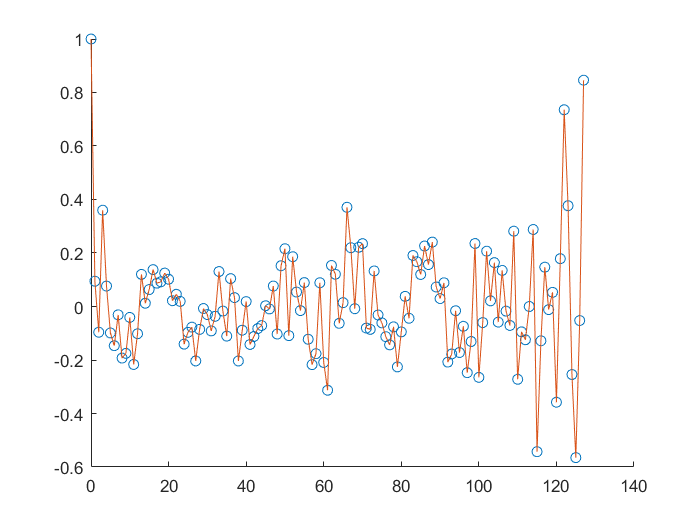
\includegraphics[scale=0.45]{../EJ1/rxxNP}
\caption{$r_{xx}(k)$ a partir del estimador no polarizado.}
\label{rxxNP}
\end{figure}

\begin{figure}[H] %!ht
\centering
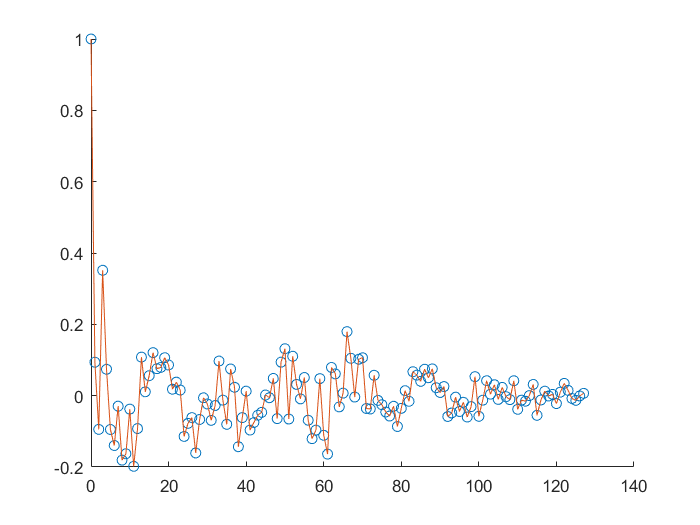
\includegraphics[scale=0.45]{../EJ1/rxxP}
\caption{$r_{xx}(k)$ a partir del estimador polarizado.}
\label{rxxP}
\end{figure}

%%
\subsection{Estimaci\'on de los primeros 127 coeficientes de correlaci\'on parcial}

\begin{figure}[H] %!ht
\centering
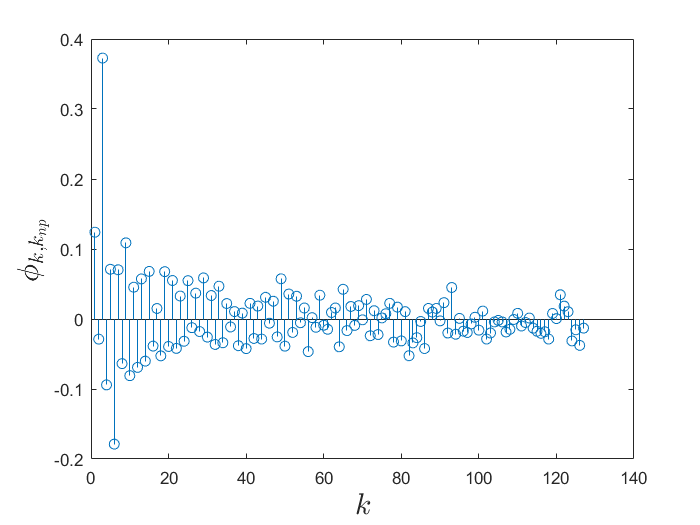
\includegraphics[scale=0.45]{../EJ1/coefCorrParcialNP}
\caption{Coeficientes de correlaci\'on parcial a partir del estimador no polarizado.}
\label{fiNP}
\end{figure}

\begin{figure}[H] %!ht
\centering
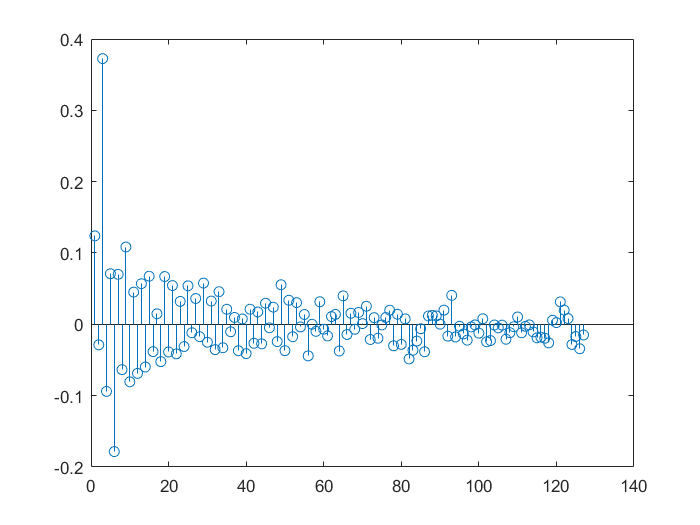
\includegraphics[scale=0.45]{../EJ1/coefCorrParcialP}
\caption{Coeficientes de correlaci\'on parcial a partir del estimador polarizado.}
\label{fiP}
\end{figure}

%%
\subsection{Determinaci\'on del modelo y orden que ajusta a la secuencia aleatoria $X(n)$}

Luego de probar con distintos modelos, se determin\'o que el que mejor ajusta a la secuencia aleatoria $X(n)$ podr\'ia ser el AR de orden 2. Teniendo en cuenta que la entrada es una secuencia de ruido blanco y Gaussiano con varianza unitaria, se hallan los par\'ametros de este modelo.

Se calcula anal\'iticamente $R_{xx}(k)$ y $ r_{xx}(k) $, con $k$ entero entre 0 y 127, para el caso del modelo AR orden 2, con las ecuaciones del libro de Shanmugan. %PONER EL NUMERO DE LAS ECUACIONES

\begin{figure}[H] %!ht
\centering
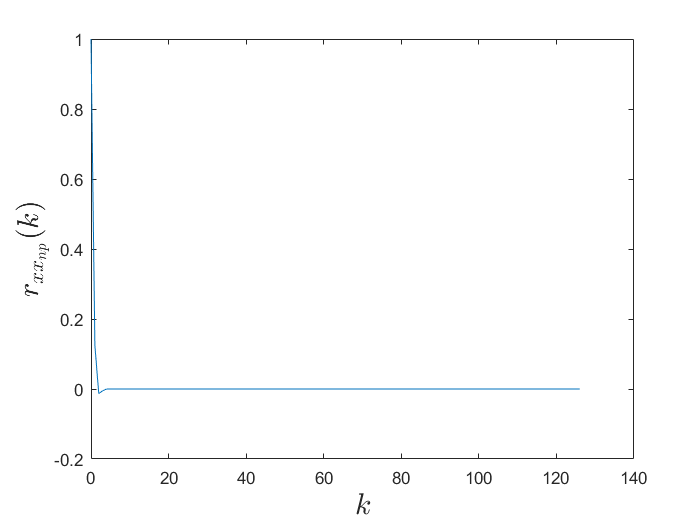
\includegraphics[scale=0.45]{../EJ1/rxxNPteorico}
\caption{$r_{xx}(k)$ a partir del estimador no polarizado, obtenido en forma teórica, en base al modelo AR orden 2.}
\label{rxxTeo}
\end{figure}
%COMPARAR ESTO CON LO ESTIMADO AL PRINCIPIO


%%
\subsection{Estimaci\'on de la densidad espectral de potencia de X(n)}

En primer lugar, se estima la densidad espectral de potencia a partir de la transformada de Fourier discreta de la autocorrelación no polarizada. Los resultados pueden observarse en la figura \ref{densidadEs}.

\begin{figure}[H] %!ht
\centering
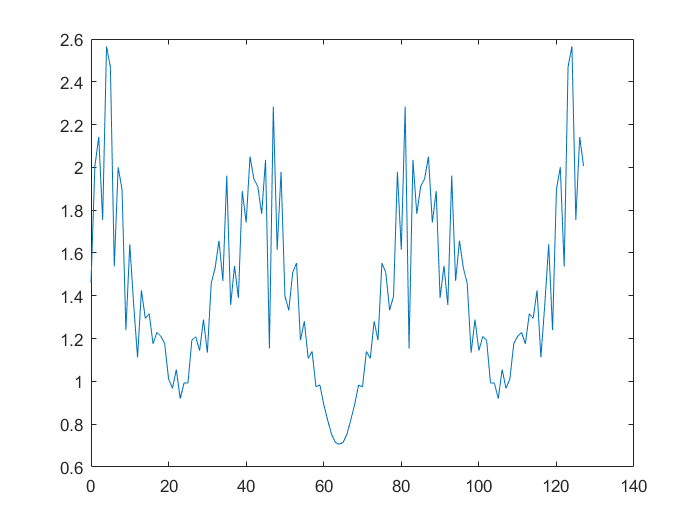
\includegraphics[scale=0.45]{../EJ1/densidadEspectralFourierDiscNP}
\caption{Estimaci\'on de la densidad espectral de potencia  de X(n) a partir de la transformada de Fourier discreta de la estimaci\'on de la autocorrelación no polarizada.}
\label{densidadEs}
\end{figure}

Por otro lado, se estima la densidad espectral de potencia a partir de la promediaci\'on de periodogramas. Pueden verse los resultados en la figura \ref{perio}.

\begin{figure}[H] %!ht
\centering
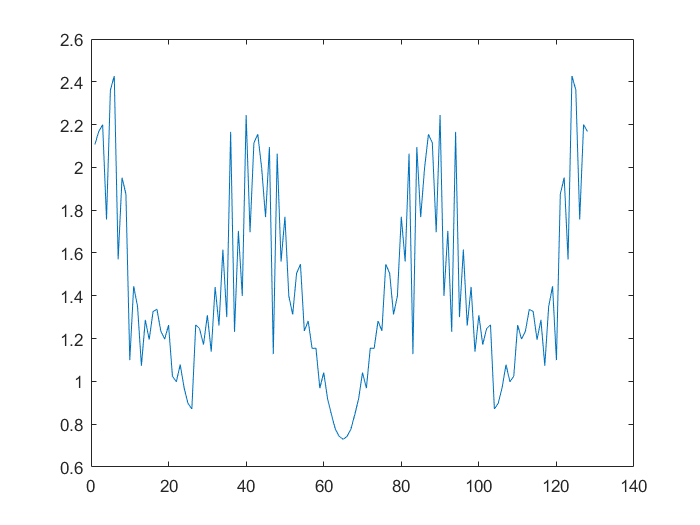
\includegraphics[scale=0.45]{../EJ1/periodogramaNP}
\caption{Estimaci\'on de la densidad espectral de potencia de $X(n)$ a partir de la promediaci\'on de periodogramas.}
\label{perio}
\end{figure}


%%%%%%%%%%%%%%%%%%%%%%%%%%%%%
\section*{Ejercicio 2}



\end{document}
